% Glucometers and Rapid Test Kits
% Compile from this folder with:  pdflatex report.tex  (run it twice)
\documentclass[11pt,a4paper]{article}

\usepackage[T1]{fontenc}
\usepackage{lmodern}
\usepackage[a4paper,margin=2cm]{geometry}
\usepackage{amsmath}
\usepackage{graphicx}
\usepackage{booktabs}
\usepackage{array}
\usepackage{xcolor}
\usepackage{caption}
\usepackage{enumitem}
\usepackage{tikz}
\usetikzlibrary{arrows.meta,positioning,calc}
\usepackage[hidelinks]{hyperref}

\graphicspath{{../outputs/}}
\captionsetup{font=small,labelfont=bf}
\setlength{\parindent}{0pt}
\setlength{\parskip}{6pt}
\setlist{nosep,leftmargin=*}

\tikzset{
  box/.style={draw,rounded corners=2pt,align=center,font=\small,inner sep=5pt},
  flow/.style={-{Stealth[length=2.2mm]},thick},
}

\newcommand{\studentname}{Aarav Gupta}

\definecolor{coverblue}{RGB}{24,62,112}

\begin{document}

% ---------------- Cover page ----------------
\begin{titlepage}
\begin{tikzpicture}[remember picture,overlay]
  \draw[coverblue,line width=2pt]
    ([shift={(1.2cm,1.2cm)}]current page.south west) rectangle ([shift={(-1.2cm,-1.2cm)}]current page.north east);
  \draw[coverblue,line width=0.5pt]
    ([shift={(1.4cm,1.4cm)}]current page.south west) rectangle ([shift={(-1.4cm,-1.4cm)}]current page.north east);
\end{tikzpicture}
\centering
\vspace*{1.2cm}

{\large\scshape Research Report}

\vfill
{\color{coverblue}\rule{0.7\linewidth}{1pt}}\\[14pt]
{\fontsize{30}{36}\selectfont\bfseries\color{coverblue} Glucometers and\\[4pt] Rapid Test Kits\par}
\vspace{12pt}
{\Large How three sciences measure blood sugar,\\[2pt] and whether it can be predicted\par}
\vspace{10pt}
{\color{coverblue}\rule{0.7\linewidth}{1pt}}

\vfill
{\large
\begin{tabular}{@{}>{\bfseries}r@{\hspace{10pt}}l@{}}
Author & \studentname\\
\end{tabular}\par}
\vspace{1.4cm}
\end{titlepage}
\setcounter{page}{1}

\section*{1. Introduction}

About 11.4\% of the people surveyed in a large national study in India had diabetes \cite{indiab}. In diabetes, the body cannot keep the amount of glucose (sugar) in the blood within safe limits. Too much sugar harms the body slowly over years, while too little can cause collapse quickly, so people with diabetes must check their level often. That number decides what they eat and how much medicine they take.

A glucometer gives this number from one drop of blood in seconds, at home, without a laboratory. Although it is small, it depends on three sciences at once: an enzyme recognises the glucose, a chemical reaction releases electrons, and an electric circuit measures them. Rapid test kits work on a similar idea: a specific chemical reaction produces a signal that a person can read.

A glucometer has one weakness. It shows what the sugar level is now, but not where it is heading, and a reading of 100\,mg/dL that is falling needs a different response from one that is rising. Sensors worn on the skin now record sugar automatically, which makes it possible to ask whether the future level can be calculated.

Sections 2 to 4 explain the physics, chemistry and biology of these devices. Section 5 connects them and describes my investigation using real patient data, and Section 6 weighs the benefits and limitations. Appendix A explains the Clarke Error Grid in more detail.

\textbf{Why I chose this topic.} I enjoy mathematics and computing, and I wanted a topic I could investigate without a laboratory. Patient data from glucose sensors is published freely, so I could test a real question myself: can blood sugar be predicted before it changes?

\section*{2. Physics principles}

Inserting a test strip connects two electrodes to the meter, forming a complete circuit (Figure~\ref{fig:strip}). The meter's battery converts chemical energy into electrical energy and applies a small, fixed voltage across the electrodes. When blood fills the strip, charge can flow, and an ammeter inside the meter, connected in series, measures the current \cite{wang}. The energy finally appears as light from the display.

Electric current is the rate of flow of charge, $I = Q/t$. Ohm's law states $V = IR$. Treating the strip as a simple resistor, with illustrative values of $V = 0.4$\,V and $I = 8\,\mu$A:
\[
R = \frac{V}{I} = \frac{0.4}{8\times10^{-6}} = 5\times10^{4}\,\Omega = 50\,\text{k}\Omega,
\qquad
P = VI = 3.2\,\mu\text{W}.
\]

If this current flows for 5 seconds, the charge is $Q = It = 40\,\mu$C. Each electron carries $1.6\times10^{-19}$\,C, so about $2.5\times10^{14}$ electrons pass through the circuit.

More glucose releases more electrons, so more current flows at the same voltage. The meter has a stored calibration that converts each current into a sugar concentration, which appears on the screen. The voltage must stay steady, because the reading depends on comparing current at a known voltage.

\begin{figure}[ht]
\centering
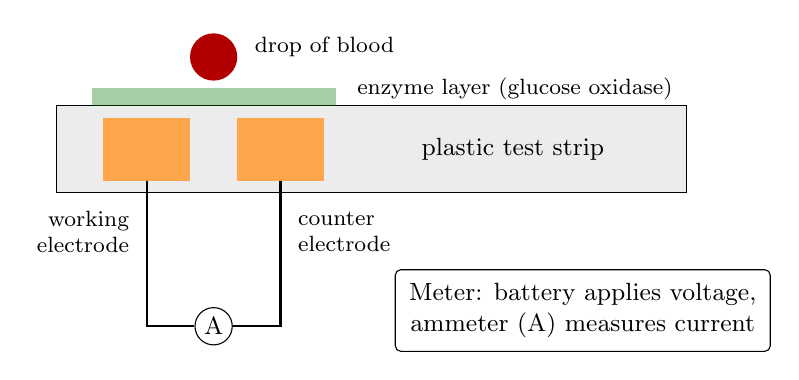
\begin{tikzpicture}[x=1cm,y=1cm]
  \fill[gray!15] (0,0) rectangle (8,1.1);
  \draw (0,0) rectangle (8,1.1);
  \node[font=\small] at (5.8,0.55) {plastic test strip};
  \fill[orange!70] (0.6,0.15) rectangle (1.7,0.95);
  \fill[orange!70] (2.3,0.15) rectangle (3.4,0.95);
  \node[font=\footnotesize,align=right,anchor=east] at (1.05,-0.5) {working\\electrode};
  \node[font=\footnotesize,align=left,anchor=west] at (2.95,-0.5) {counter\\electrode};
  \fill[green!45!black,opacity=.35] (0.45,1.1) rectangle (3.55,1.32);
  \node[font=\footnotesize,anchor=west] at (3.7,1.32) {enzyme layer (glucose oxidase)};
  \fill[red!70!black] (2,1.72) circle (0.3);
  \node[font=\footnotesize,anchor=west] at (2.4,1.85) {drop of blood};
  \node[draw,circle,inner sep=1.5pt,font=\small] (a) at (2,-1.7) {A};
  \draw[thick] (1.15,0.15) -- (1.15,-1.7) -- (a.west);
  \draw[thick] (2.85,0.15) -- (2.85,-1.7) -- (a.east);
  \node[box,anchor=west] at (4.3,-1.5) {Meter: battery applies voltage,\\ammeter (A) measures current};
\end{tikzpicture}
\caption{A glucose test strip as an electric circuit (own diagram, simplified).}
\label{fig:strip}
\end{figure}

\section*{3. Chemistry principles}

The strip contains the enzyme glucose oxidase. An enzyme is a biological catalyst: it speeds up a reaction without being used up. This one is specific, meaning it reacts with glucose but almost nothing else, which is why other sugars and substances in blood have little effect. In the classic reaction, glucose is oxidised to gluconic acid while oxygen is reduced to hydrogen peroxide. Counting atoms on each side (6 C, 14 H and 9 O) shows that the equation is balanced:
\[
\mathrm{C_6H_{12}O_6 + O_2 + H_2O \;\longrightarrow\; C_6H_{12}O_7 + H_2O_2}
\]
The hydrogen peroxide formed is then oxidised at the anode, giving up electrons:
\[
\mathrm{H_2O_2 \;\longrightarrow\; O_2 + 2H^+ + 2e^-}
\]
As in electrolysis, oxidation (loss of electrons) happens at the anode, and those electrons form the current that the meter measures. Reduction at the other electrode completes the circuit, and dissolved ions in the blood carry charge between the electrodes, so blood acts as the electrolyte. Many modern strips replace oxygen with a mediator such as ferricyanide, which carries electrons from the enzyme to the electrode \cite{wang}.

\textbf{Mole calculation.} The molar mass of glucose is $6(12)+12(1)+6(16)=180$\,g/mol. A reading of 126\,mg/dL equals 1.26\,g/L, so
\[
\text{concentration} = \frac{1.26\ \text{g/L}}{180\ \text{g/mol}} = 0.007\ \text{mol/L} = 7\ \text{mmol/L},
\]
which is the World Health Organization's fasting threshold for diagnosing diabetes \cite{who}.

\section*{4. Biology principles}

Digestion breaks carbohydrates down into glucose, which is absorbed in the small intestine, enters the blood and is carried to every cell for respiration. The pancreas acts as an endocrine gland: groups of cells called the islets of Langerhans release hormones directly into the blood, and these control the sugar level (Figure~\ref{fig:loop}). When sugar is high, beta cells release \textbf{insulin}, which makes cells take up glucose and the liver store it as glycogen. When sugar is low, alpha cells release \textbf{glucagon}, which makes the liver turn glycogen back into glucose. Each response corrects the change that triggered it, so this is negative feedback.

\begin{figure}[ht]
\centering
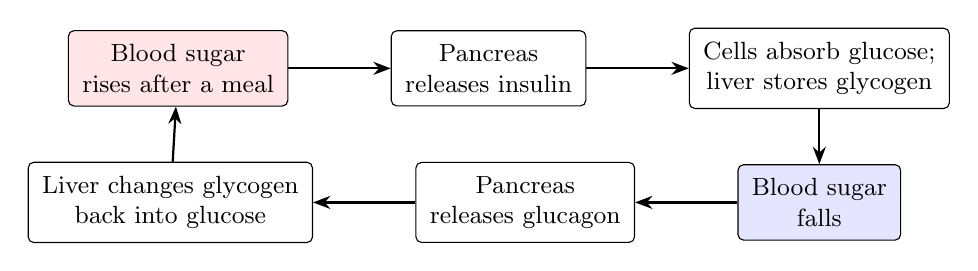
\begin{tikzpicture}[node distance=7mm and 13mm]
  \node[box,fill=red!10] (high) {Blood sugar\\rises after a meal};
  \node[box,right=of high] (ins) {Pancreas\\releases insulin};
  \node[box,right=of ins] (store) {Cells absorb glucose;\\liver stores glycogen};
  \node[box,fill=blue!10,below=of store] (low) {Blood sugar\\falls};
  \node[box,left=of low] (glu) {Pancreas\\releases glucagon};
  \node[box,left=of glu] (rel) {Liver changes glycogen\\back into glucose};
  \draw[flow] (high) -- (ins);
  \draw[flow] (ins) -- (store);
  \draw[flow] (store) -- (low);
  \draw[flow] (low) -- (glu);
  \draw[flow] (glu) -- (rel);
  \draw[flow] (rel) -- (high);
\end{tikzpicture}
\caption{Negative feedback control of blood sugar (own diagram).}
\label{fig:loop}
\end{figure}

In Type 1 diabetes, the body's immune system destroys the cells that make insulin. In Type 2 diabetes, which is far more common, body cells respond poorly to insulin (insulin resistance), and over time the pancreas may not make enough. Sugar then stays high for hours, which damages blood vessels, eyes, kidneys and nerves. Sugar below about 70\,mg/dL is also dangerous, and can cause shaking, confusion or unconsciousness. Treatment combines diet, exercise, tablets and insulin injections, and regular testing shows whether it is working.

\section*{5. How the sciences work together, and my investigation}

\textbf{Biology} explains why sugar must be measured. \textbf{Chemistry} turns glucose into electrons. \textbf{Physics} turns electrons into a number. None of them works without the others: without the enzyme there is no signal, without the circuit no reading, and without the biology the reading has no meaning.

Many rapid test kits show the same link. A liquid sample moves along a paper strip by capillary action (physics). Antibodies, which are proteins made to fit one target (biology), are attached to coloured particles and bind to that target by specific chemical interactions (chemistry). A visible line then appears, so the kit needs no electricity at all.

\textbf{Research question.} Can sugar be predicted 30 and 60 minutes ahead for Type 2 patients a computer has never seen, and does adding the body's equations help?

\textbf{Data.} I used the public ShanghaiT2DM dataset \cite{zhao}: 100 patients and 112,475 sensor readings taken every 15 minutes, with their meals and medicines (Figure~\ref{fig:patient}). I estimated each meal's carbohydrates from its food list. For example, cooked rice is about 26\% carbohydrate, so 150\,g of rice contains $150 \times 26 / 100 = 39$\,g.

\begin{figure}[ht]
\centering
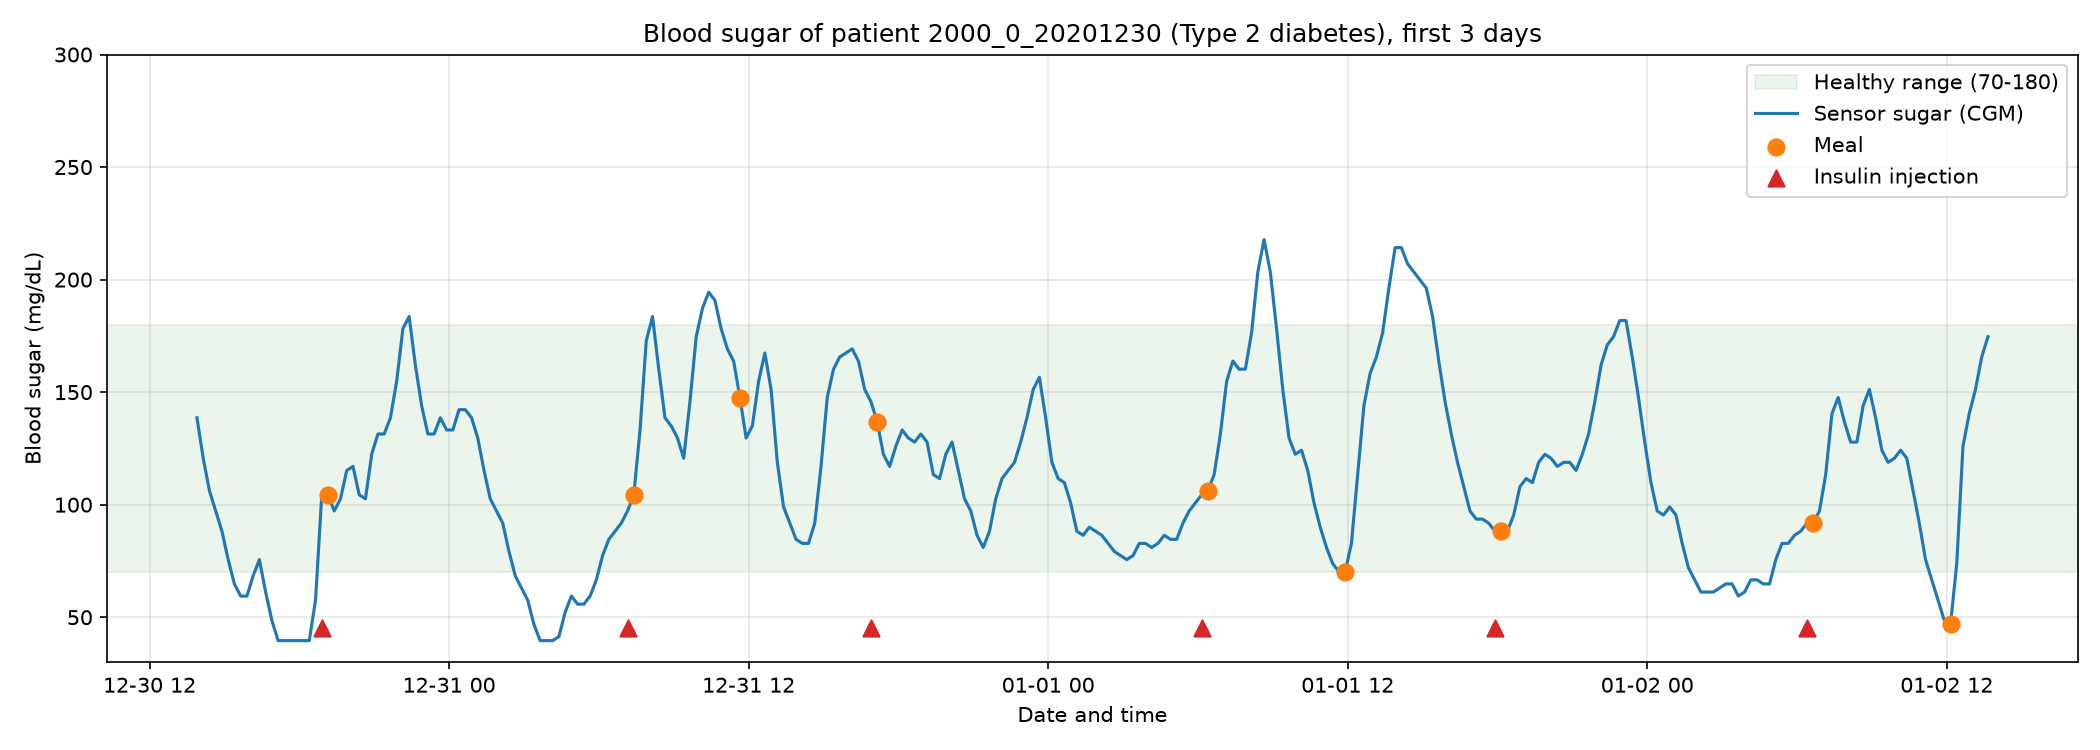
\includegraphics[width=0.92\linewidth]{2000_0_20201230.png}
\caption{Three days of real data from one patient \cite{zhao}. Sugar tends to rise after meals and fall after insulin (own graph).}
\label{fig:patient}
\end{figure}

\textbf{The equations.} The Bergman model \cite{bergman} treats blood sugar like water in a bathtub (Figure~\ref{fig:tub}). Every minute,
\[
\text{new sugar} = \text{old sugar} + \text{food} - \text{natural return to normal} - \text{effect of insulin}.
\]
Repeating this step 30 or 60 times gives a forecast.

\begin{figure}[ht]
\centering
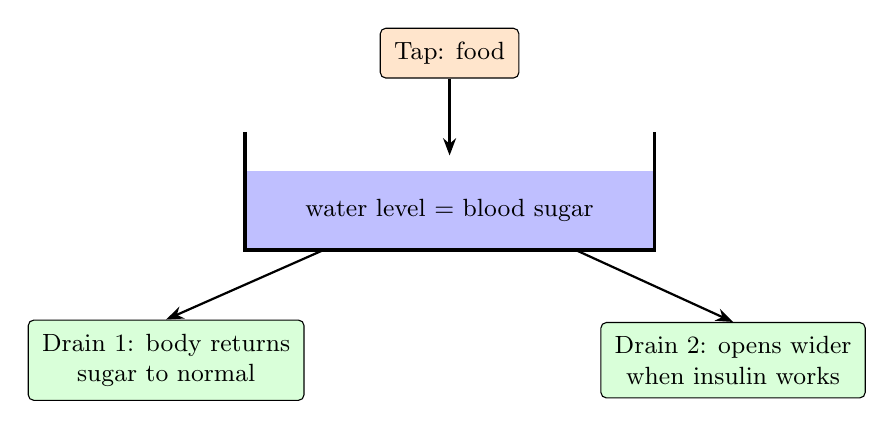
\begin{tikzpicture}[x=1cm,y=1cm]
  \node[box,fill=orange!20] (tap) at (0,2.5) {Tap: food};
  \fill[blue!25] (-2.6,0) rectangle (2.6,1);
  \draw[very thick] (-2.6,1.5) -- (-2.6,0) -- (2.6,0) -- (2.6,1.5);
  \node[font=\small] at (0,0.5) {water level = blood sugar};
  \draw[flow] (tap) -- (0,1.2);
  \node[box,fill=green!15] (d1) at (-3.6,-1.4) {Drain 1: body returns\\sugar to normal};
  \node[box,fill=green!15] (d2) at (3.6,-1.4) {Drain 2: opens wider\\when insulin works};
  \draw[flow] (-1.6,0) -- (d1.north);
  \draw[flow] (1.6,0) -- (d2.north);
\end{tikzpicture}
\caption{The ``bathtub'' picture of the model (own diagram).}
\label{fig:tub}
\end{figure}

\textbf{Method.} Four methods competed. The \emph{Lazy Guess} assumes sugar will not change. The \emph{Equations} use the model above. The \emph{Pattern Learner} is a machine-learning model (XGBoost \cite{xgboost}) that learns from past examples. The \emph{Hybrid} is the Pattern Learner given the Equations' forecast as extra information. The models learned from 80 patients and were tested on 20 others. Separating patients this way keeps the test fair, because a model cannot simply memorise someone it has already seen. A plain average treats all mistakes as equal, but guessing 190 when the truth is 50 is far worse than guessing 190 when the truth is 170. So errors were also graded with the Clarke Error Grid \cite{clarke} (Appendix A), where Zone A means accurate and Zone D means a dangerous reading was missed.

\begin{table}[ht]
\centering
\caption{Results on 19,813 moments from 20 unseen patients. Error is the average in mg/dL.}
\label{tab:results}
\begin{tabular}{@{}lrrrrrr@{}}
\toprule
& \multicolumn{3}{c}{30 minutes ahead} & \multicolumn{3}{c}{60 minutes ahead}\\
\cmidrule(lr){2-4}\cmidrule(l){5-7}
Method & Error & Zone A & Zone D & Error & Zone A & Zone D\\
\midrule
Lazy Guess      & 12.42 & 90.78\% & 0.51\% & 21.46 & 74.63\% & 1.59\%\\
Equations       & 11.56 & 92.62\% & 0.48\% & 19.22 & 79.09\% & 1.48\%\\
Pattern Learner &  9.37 & 95.29\% & 0.76\% & 17.01 & 81.81\% & 1.98\%\\
\textbf{Hybrid} & \textbf{9.20} & \textbf{95.91\%} & 0.63\% & \textbf{16.51} & \textbf{82.74\%} & 1.96\%\\
\bottomrule
\end{tabular}
\end{table}

\begin{figure}[ht]
\centering
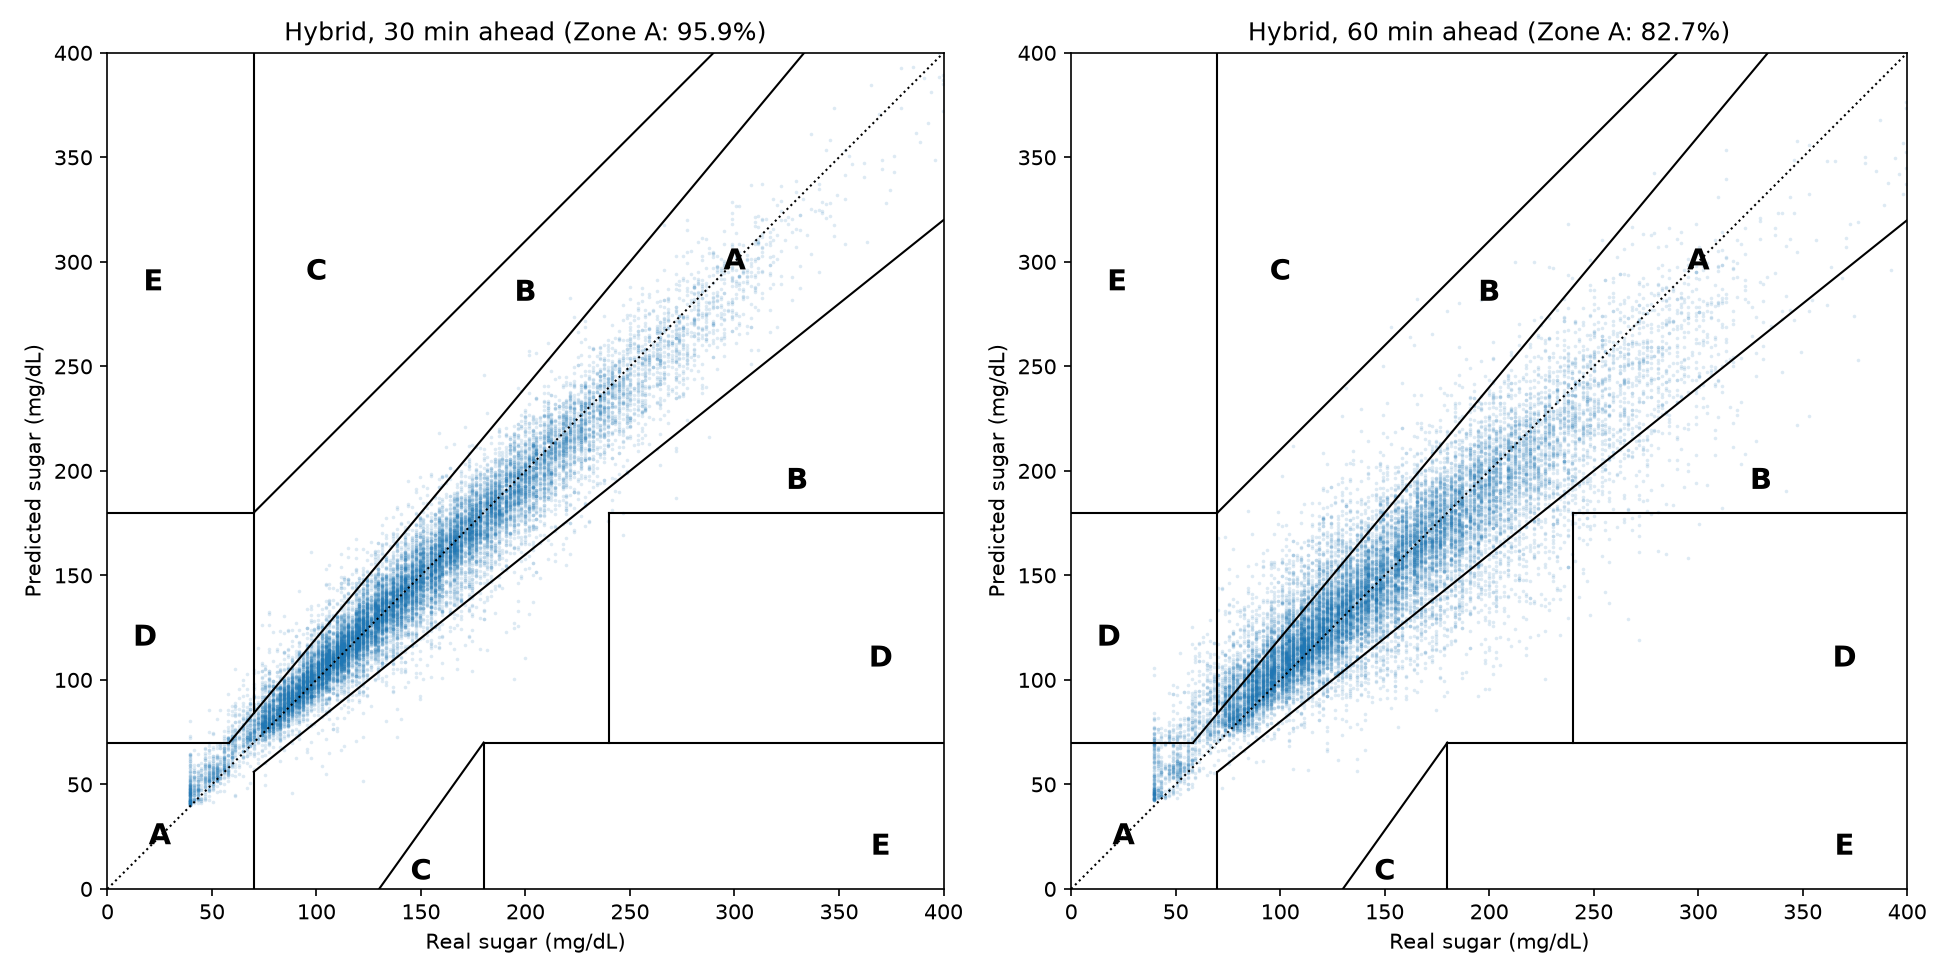
\includegraphics[width=0.86\linewidth]{clarke_hybrid.png}
\caption{Clarke Error Grids for the Hybrid. Each dot is one prediction (own graph).}
\label{fig:clarke}
\end{figure}

\textbf{Findings.} The Hybrid was the most accurate (Table~\ref{tab:results}, Figure~\ref{fig:clarke}), with about a quarter less error than the Lazy Guess, and it beat the Lazy Guess on all 20 patients. Its gain over the Pattern Learner alone was small: 0.17\,mg/dL at 30 minutes (better on 14 of 20 patients) and 0.47\,mg/dL at 60 minutes (better on 15 of 20). However, the Equations missed the fewest dangerous readings. When sugar really was low, the machine-learning models guessed too high on average, which is the risky direction.

\section*{6. Benefits, limitations and conclusion}

{\small
\noindent\begin{tabular}{@{}>{\bfseries}p{2.4cm}p{6.3cm}p{6.3cm}@{}}
\toprule
& \textbf{Benefits} & \textbf{Limitations}\\
\midrule
People & Fast readings at home; safer decisions about food and medicine. & Finger pricks are painful; other substances in blood can disturb readings \cite{wang}. \\
Society & Earlier care may prevent costly emergencies. & Strips are a repeated cost, and access is unequal. \\
Environment & Home testing can reduce trips to clinics. & Used strips, lancets and batteries add plastic and biomedical waste. \\
\bottomrule
\end{tabular}
}

\textbf{Limits of my study.} Only 20 patients were tested, all from one region of China. Carbohydrates were rough estimates. The Equations failed on their first attempt (23.50\,mg/dL error at 30 minutes) and were corrected using practice patients, so the 20 test patients were used twice for them, and the Hybrid depends on that corrected version. The learned values do not represent true body measurements, and none of these models is a medical device.

\textbf{Conclusion.} A glucometer shows how three sciences depend on each other: biology creates the need, chemistry creates the signal and physics makes it readable. Remove any one of them and the device is no longer useful.

My investigation asked whether sugar can be predicted, and the answer is yes, to a limited extent. The Hybrid's average error was 9.20\,mg/dL at 30 minutes, against 12.42 for assuming no change, and 16.51 at 60 minutes, against 21.46. Error grew considerably with a longer forecast, so the further ahead a prediction looks, the less it can be trusted. Adding the equations helped only slightly, although a patient-by-patient Wilcoxon test (p = 0.027 at 30 minutes and p = 0.002 at 60 minutes) suggests that this small gain was unlikely to be pure chance.

The most important finding was about safety. When real sugar was below 70\,mg/dL, the Hybrid guessed on average 7.46\,mg/dL too high at 30 minutes and 15.99 at 60 minutes, compared with 3.71 and 8.53 for the Equations. The most accurate model was therefore not the safest at dangerous lows, so a prediction system should be judged on safety as well as average accuracy. With more time, I would test patients from more regions, use carefully measured meals, and train the model to treat mistakes at low sugar as more serious.

\textbf{Acknowledgement of AI use.} I used Claude (Anthropic) to aid in writing the code and drafting the report.

\begin{thebibliography}{9}
\small
\setlength{\itemsep}{1pt}
\bibitem{indiab} Anjana RM, et al. Metabolic non-communicable disease health report of India: the ICMR-INDIAB national cross-sectional study. \emph{Lancet Diabetes Endocrinol.} 2023;11(7):474--489.
\bibitem{wang} Wang J. Glucose biosensors: 40 years of advances and challenges. \emph{Electroanalysis.} 2001;13(12):983--988.
\bibitem{who} World Health Organization. \emph{Definition and diagnosis of diabetes mellitus and intermediate hyperglycaemia.} Geneva: WHO; 2006.
\bibitem{zhao} Zhao Q, et al. Chinese diabetes datasets for data-driven machine learning. \emph{Sci Data.} 2023;10:35.
\bibitem{bergman} Bergman RN, Ider YZ, Bowden CR, Cobelli C. Quantitative estimation of insulin sensitivity. \emph{Am J Physiol.} 1979;236(6):E667--E677.
\bibitem{xgboost} Chen T, Guestrin C. XGBoost: a scalable tree boosting system. \emph{Proc. KDD.} 2016:785--794.
\bibitem{clarke} Clarke WL, Cox D, Gonder-Frederick LA, Carter W, Pohl SL. Evaluating clinical accuracy of systems for self-monitoring of blood glucose. \emph{Diabetes Care.} 1987;10(5):622--628.
\end{thebibliography}

\section*{Appendix A: The Clarke Error Grid}

The simplest score is the mean absolute error (MAE), the average size of the mistakes:
\[
\text{MAE} = \frac{1}{n}\sum_{i=1}^{n}\bigl|\,\text{guess}_i - \text{truth}_i\,\bigr|.
\]
If the guesses are 110 and 150 and the truths are 100 and 180, then MAE $= (10+30)/2 = 20$\,mg/dL. Its flaw is that it treats all mistakes of the same size as equally serious. Guessing 110 when the truth is 50 hides a dangerous low, while guessing 240 when the truth is 180 changes little, yet both are errors of 60.

Clarke and colleagues \cite{clarke} solved this by plotting each prediction as a point, with the true sugar $t$ on the $x$-axis and the guess $g$ on the $y$-axis. A perfect prediction lies on the line $y = x$. The graph is divided into five zones according to what a patient would do if they trusted the guess (Table~\ref{tab:zones}). The boundaries at 70 and 180\,mg/dL mark the edges of the target range, so a guess on the wrong side of one changes the treatment.

\begin{table}[ht]
\centering
\small
\caption{The five zones, as coded in my program. The rules are tested in the order A, E, C, D, and anything left over is B.}
\label{tab:zones}
\begin{tabular}{@{}l>{\raggedright\arraybackslash}p{6.7cm}>{\raggedright\arraybackslash}p{4.9cm}l@{}}
\toprule
Zone & Rule & Meaning & $t \to g$\\
\midrule
A & $g$ within 20\% of $t$, or both at most 70 & Accurate enough to treat correctly & $200 \to 170$\\
B & None of the other rules applies & Wrong, but the treatment would be harmless & $200 \to 250$\\
C & $70 \le t \le 290$ and $g \ge t+110$; or $130 \le t \le 180$ and $g \le 1.4t-182$ & Overcorrection: an acceptable sugar level gets ``treated'' & $100 \to 220$\\
D & $g$ between 70 and 180 while $t \ge 240$ or $t \le 58.3$; or $58.3 \le t \le 70$ and $g \ge 1.2t$ & A dangerous level is missed & $50 \to 100$\\
E & $t \ge 180$ and $g \le 70$; or $t \le 70$ and $g \ge 180$ & Opposite treatment: high is read as low, or low as high & $250 \to 60$\\
\bottomrule
\end{tabular}
\end{table}

For example, 20\% of 200 is 40, so Zone A runs from 160 to 240, and a guess of 170 is in Zone A. For the Hybrid at 30 minutes, 95.91\% of the 19,813 predictions (about 19,000) were in Zone A and 0.63\% (about 125) were in Zone D. A small percentage still matters, because each Zone D point is a moment when danger would have been missed. The grid was designed to grade meters that measure sugar now, so using it on forecasts is my adaptation.

\end{document}
